%%%%%%%%%%%%%%%%%%%%%%%%%%%%%%%%%%%%%%%%%
% a0poster Portrait Poster — Blank Template
% Based on the a0poster class by Kettl & Weiser
% License: CC BY-NC-SA 3.0
%%%%%%%%%%%%%%%%%%%%%%%%%%%%%%%%%%%%%%%%%

%-------------------------------------------------------------------------------
%	PACKAGES AND OTHER DOCUMENT CONFIGURATIONS
%-------------------------------------------------------------------------------

\documentclass[a0, portrait]{a0poster}

\usepackage{multicol}
\columnsep=100pt
\columnseprule=3pt

\usepackage[svgnames]{xcolor}
\usepackage{palatino}
\usepackage{graphicx}
\graphicspath{{figures/}}
\usepackage{float}
\usepackage{tikz}
\usetikzlibrary{positioning, arrows.meta, shadows, shadings}
\usetikzlibrary{shapes.geometric, positioning, fit, backgrounds, shadows, decorations.pathmorphing, calc, arrows.meta}
\usepackage{tikzscale}
\usepackage{booktabs}
\usepackage[font=small,labelfont=bf]{caption}
\usepackage{amsfonts, amsmath, amsthm, amssymb}
\usepackage{wrapfig}
\usepackage{url}

%-------------------------------------------------------------------------------
%  FIGURE PLACEHOLDER COMMAND
%  Usage: \figplaceholder[height]{label text}
%  Replace with \includegraphics when you have real figures.
%  Default height is 8cm; pass an optional first argument to change it.
%-------------------------------------------------------------------------------
\newcommand{\figplaceholder}[2][8cm]{%
  \noindent
  \colorbox{lightgray!40}{%
    \begin{minipage}[c][#1][c]{\linewidth}
      \centering
      \color{gray}\large [Figure: #2]
    \end{minipage}%
  }%
}

%-------------------------------------------------------------------------------
%  LOGO PLACEHOLDER COMMAND
%  Usage: \logoplaceholder{width}{label}
%-------------------------------------------------------------------------------
\newcommand{\logoplaceholder}[2]{%
  \colorbox{lightgray!40}{%
    \begin{minipage}[c][#1][c]{#1}
      \centering
      \color{gray}\small [#2]
    \end{minipage}%
  }%
}

\newcommand{\av}{anat2vess }
\newcommand{\postertitle}[1]{%
  {\Huge\bfseries\color{NavyBlue}%
   \setlength{\baselineskip}{70pt}%
   #1\par}%
}

\begin{document}

%----------------------------------------------------------------------------------------
%	POSTER HEADER
%----------------------------------------------------------------------------------------

% Header: two boxes.
%   Left  (90%): title, authors, affiliations, contact.
%   Right (10%): institution logo.

\begin{minipage}[b]{0.9\linewidth}
  \veryHuge \color{NavyBlue} \textbf{Vessels hiding in plain sight: quantifying brain
vascular morphology in anatomical MRI
using deep learning} \color{Black}\\
  \huge \textbf{Asa Gilmore\textsuperscript{1, 2},
  Anita Esi Eshun\textsuperscript{3},
  Yue Wu \textsuperscript{4, 5},
  Aaron Lee\textsuperscript{4, 5},
  \& Ariel Rokem \textsuperscript{1, 2*}}\\
  \Large 1. Dept. of Physics, Univ. of Washington,
         2. The eScience Institute,
         3. Kumasi Centre for Collaborative Research, \\
         4. Department of Ophthalmology, University of Washington,
         5. Roger and Angie Karalis Johnson Retina Center, University of Washington \\
  \Large Contact: \texttt{arokem@uw.edu}
         $|$ Download: \texttt{}
\end{minipage}
%
\begin{minipage}[b]{0.1\linewidth}
  % Replace \logoplaceholder with:
    
\includegraphics[width=8cm]{UWlogo.png}
    
\includegraphics[width=8cm]{camh_logo.png}
%   \logoplaceholder{10cm}{Logo}
\end{minipage}

\vspace{0.5cm}

%----------------------------------------------------------------------------------------

\begin{multicols}{2}

%----------------------------------------------------------------------------
%	INTRODUCTION
%----------------------------------------------------------------------------

\section*{Introduction}

Non-invasive measurements of brain blood vessels with magnetic
resonance angiography (MRA) provide important information about brain health
and aging. But MRA is time-consuming and is not as commonly used as anatomical
MRI contrasts. We trained a neural network model on paired MRI/MRA scans to
accurately delineate major blood vessels and we derived vessel morphology
features that account for as much as 78\% of the variance in MRA-derived
features. The model generalized well in two other datasets, where we found that
model-based vessel morphology features contain information about aging, and are
associated with individual variability in blood pressure, cognitive decline and
Alzheimer's dementia. These results demonstrate that our model could be useful
in a range of existing and new datasets to assess the role of brain blood
vessels in aging and in brain health. The methods are provided as open-source
software at https://github.com/nrdg/anat2vessels.

\rule{\linewidth}{0.4pt}

%----------------------------------------------------------------------------
%	MATERIALS AND METHODS
%----------------------------------------------------------------------------

\normalsize
\section*{Materials and Methods}

\subsection*{Dataset}
We used the publicly available IXI dataset (\url{http://brain-development.org/ixi-dataset/}),
containing T1w, T2w, and MRA for N=567 subjects.

During training the dataset was randomly split into train (N=427) and test (N=106)
samples, following the standard nnUNet procedure using 5-fold cross-validation,
stratified by scanner.

Instead of using the raw MRA images as labels, we used
COSTA (xxx Cite), a pretrained model for segmenting blood vessels in MRA, to produce binary
vessel masks from the MRA images to use as training labels.


\subsection*{Model / Algorithm}

We used the popular (xxx cite) nnUNet architecture, implementing their nnUNet ResEnc L
model, trained with Dice and BCE loss.

\begin{minipage}[b]{\linewidth}

  \centering
  \makebox[\textwidth][c]{%
  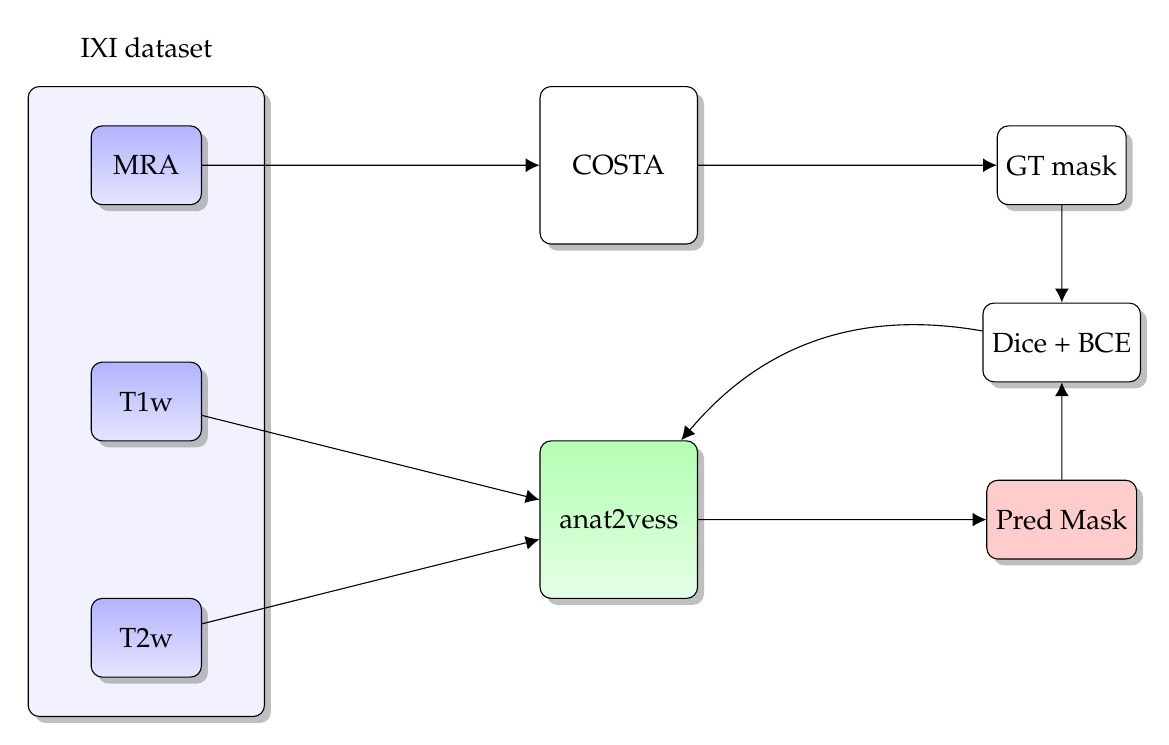
\begin{tikzpicture}[scale=1.5]
    \node at (1,6) {IXI dataset};
    \node[draw, fill=blue!5, rounded corners, minimum width=3cm, minimum height=8cm, drop shadow] at (1,3) {};

    \node[draw, fill=blue!20, top color=blue!30, bottom color=blue!10, rounded corners, minimum width=1.4cm, minimum height=1cm, drop shadow] at (1,5) (mra) {MRA};
    \node[draw, fill=blue!20, top color=blue!30, bottom color=blue!10, rounded corners, minimum width=1.4cm, minimum height=1cm, drop shadow] at (1,3) (t1w) {T1w};
    \node[draw, fill=blue!20, top color=blue!30, bottom color=blue!10, rounded corners, minimum width=1.4cm, minimum height=1cm, drop shadow] at (1,1) (t2w) {T2w};

    \node[draw, fill=white, rounded corners, minimum width=2cm, minimum height=2cm, drop shadow] at (5,5) (costa) {COSTA};
    \node[draw, fill=green!20, top color=green!30, bottom color=green!10, rounded corners, minimum width=2cm, minimum height=2cm, drop shadow] at (5,2) (nn) {\av};

    \node[draw, fill=white, rounded corners, minimum width=1.5cm, minimum height=1cm, drop shadow] at (8.75,5) (gtmask) {GT mask};
    \node[draw, fill=white, rounded corners, minimum width=1.5cm, minimum height=1cm, drop shadow] at (8.75,3.5) (loss) {Dice + BCE};
    \node[draw, fill=red!20, rounded corners, minimum width=1.5cm, minimum height=1cm, drop shadow] at (8.75,2) (predmask) {Pred Mask};

    \draw[arrows = {-Latex[width=5pt, length=5pt]}] (mra) -- (costa);
    \draw[arrows = {-Latex[width=5pt, length=5pt]}] (t1w) -- (nn);
    \draw[arrows = {-Latex[width=5pt, length=5pt]}] (t2w) -- (nn);

    \draw[arrows = {-Latex[width=5pt, length=5pt]}] (costa) -- (gtmask);
    \draw[arrows = {-Latex[width=5pt, length=5pt]}] (nn) -- (predmask);
    \draw[arrows = {-Latex[width=5pt, length=5pt]}] (gtmask) -- (loss);
    \draw[arrows = {-Latex[width=5pt, length=5pt]}] (predmask) -- (loss);
    \draw[arrows = {-Latex[width=5pt, length=5pt]}, bend right] (loss) to (nn);
  \end{tikzpicture}
  }
%  \captionsetup{labelformat=empty}

%   \caption{The~\av training pipeline.}

%   % Replace \figplaceholder with \includegraphics[width=\linewidth]{your-figure.png}
%   \figplaceholder[10cm]{Model architecture or pipeline}
  \captionof{figure}{~\av  training pipeline}
\end{minipage}
\\

\subsection*{Downstream Analysis}

In downstream analysis, the training losses of Dice and BCE fail to provide a
picture of the anatomical accuracy of the model (XXX awkward wording fix).
To evaluate the accuracy we implemented the following extraction of anatomical features
from the vessel masks: Branch length, Bifurcation Count, Endpoint Count, Vessel Radii, Vessel volume, and Branch Count.



\begin{minipage}[b]{\linewidth}
  \centering
  \makebox[\textwidth][c]{%
    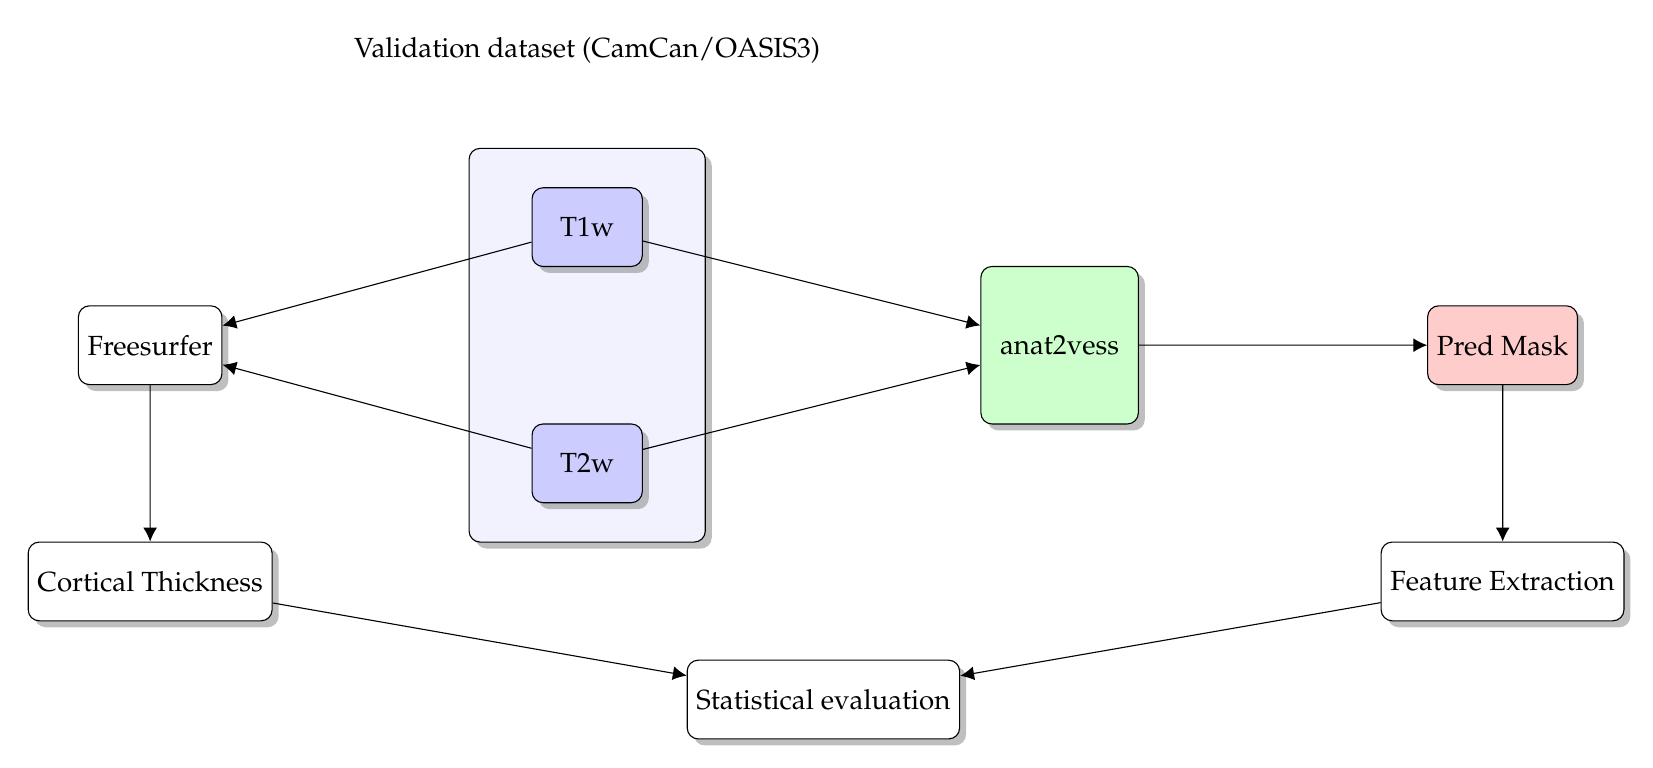
\begin{tikzpicture}[scale=1.5]
      % Main container box on the left
      \node at (1,4.5) {Validation dataset (CamCan/OASIS3)};
      \node[draw, fill=blue!5, rounded corners, minimum width=3cm, minimum height=5cm, drop shadow] at (1,2) {};

      \node[draw, fill=blue!20, rounded corners, minimum width=1.4cm, minimum height=1cm, drop shadow] at (1,3) (t1w) {T1w};
      \node[draw, fill=blue!20, rounded corners, minimum width=1.4cm, minimum height=1cm, drop shadow] at (1,1) (t2w) {T2w};
      \node[draw, fill=green!20, rounded corners, minimum width=2cm, minimum height=2cm, drop shadow] at (5,2) (nn) {\av};
      \node[draw, fill=red!20, rounded corners, minimum width=1.5cm, minimum height=1cm, drop shadow] at (8.75,2) (predmask) {Pred Mask};
      \node[draw, fill=white, rounded corners, minimum width=1.5cm, minimum height=1cm, drop shadow] at (8.75,0) (feature) {Feature Extraction};
      \node[draw, fill=white, rounded corners, minimum width=1.5cm, minimum height=1cm, drop shadow] at (-2.7,2) (fs) {Freesurfer};
      \node[draw, fill=white, rounded corners, minimum width=1.5cm, minimum height=1cm, drop shadow] at (-2.7,0) (ct) {Cortical Thickness};
      \node[draw, fill=white, rounded corners, minimum width=1.5cm, minimum height=1cm, drop shadow] at (3,-1) (stats) {Statistical evaluation};

      \draw[arrows = {-Latex[width=5pt, length=5pt]}] (t1w) -- (nn);
      \draw[arrows = {-Latex[width=5pt, length=5pt]}] (t2w) -- (nn);
      \draw[arrows = {-Latex[width=5pt, length=5pt]}] (nn) -- (predmask);
      \draw[arrows = {-Latex[width=5pt, length=5pt]}] (predmask) -- (feature);
      \draw[arrows = {-Latex[width=5pt, length=5pt]}] (t1w) -- (fs);
      \draw[arrows = {-Latex[width=5pt, length=5pt]}] (t2w) -- (fs);
      \draw[arrows = {-Latex[width=5pt, length=5pt]}] (fs) -- (ct);

      \draw[arrows = {-Latex[width=5pt, length=5pt]}] (ct) -- (stats);
      \draw[arrows = {-Latex[width=5pt, length=5pt]}] (feature) -- (stats);
    \end{tikzpicture}
  }
    \captionof{figure}{Validation Pipeline}
\end{minipage}

For validation, we use two separate datasets, CamCan, which does not contain
ground truth MRA, and OASIS3, which contains MRA, as well as T1w, and T2w scans,
within one year from cognitive assessments.

\subsection*{Acknowledgements}
\footnotesize This work was funded by National Institutes of Health grants MH121868,
MH121867, EB027585, R01AG060942, and U19AG066567, as well as by National
Science Foundation grant 1934292 and by Research to Prevent Blindness.

Preliminary testing for this work was completed on Hyak, UW’s high performance
computing cluster. This resource was funded by the UW student technology fee.

Data collection and sharing for this project was provided by the Cambridge
Centre for Ageing and Neuroscience (CamCAN). CamCAN funding was provided by the
UK Biotechnology and Biological Sciences Research Council (grant number
BB/H008217/1), together with support from the UK Medical Research Council and
University of Cambridge, UK.

Data were provided in part by OASIS: OASIS-3: Longitudinal Multimodal
Neuroimaging: Principal Investigators: T. Benzinger, D. Marcus, J. Morris; NIH
P30 AG066444, P50 AG00561, P30 NS09857781, P01 AG026276, P01 AG003991, R01
AG043434, UL1 TR000448, R01 EB009352.

Thanks to Kendrick Kay and Aviv Mezer for helpful discussions of this work.
% Funder logos — replace \logoplaceholder with \includegraphics when ready:
% \logoplaceholder{2.6cm}{Funder 1}
% \logoplaceholder{2.6cm}{Funder 2}

\columnbreak

%----------------------------------------------------------------------------
%	RESULTS
%----------------------------------------------------------------------------

\color{Navy}
\section*{Results}

\subsection*{Training Results}

Summarize your primary finding here. Explain what the model learned or what the analysis
revealed, and why it is noteworthy. Quantify the result where possible (e.g., accuracy,
error reduction, p-value).

\begin{minipage}[b]{1.0\linewidth}
  % Replace with \includegraphics[width=\linewidth]{main-result.png}
  \begin{center}

    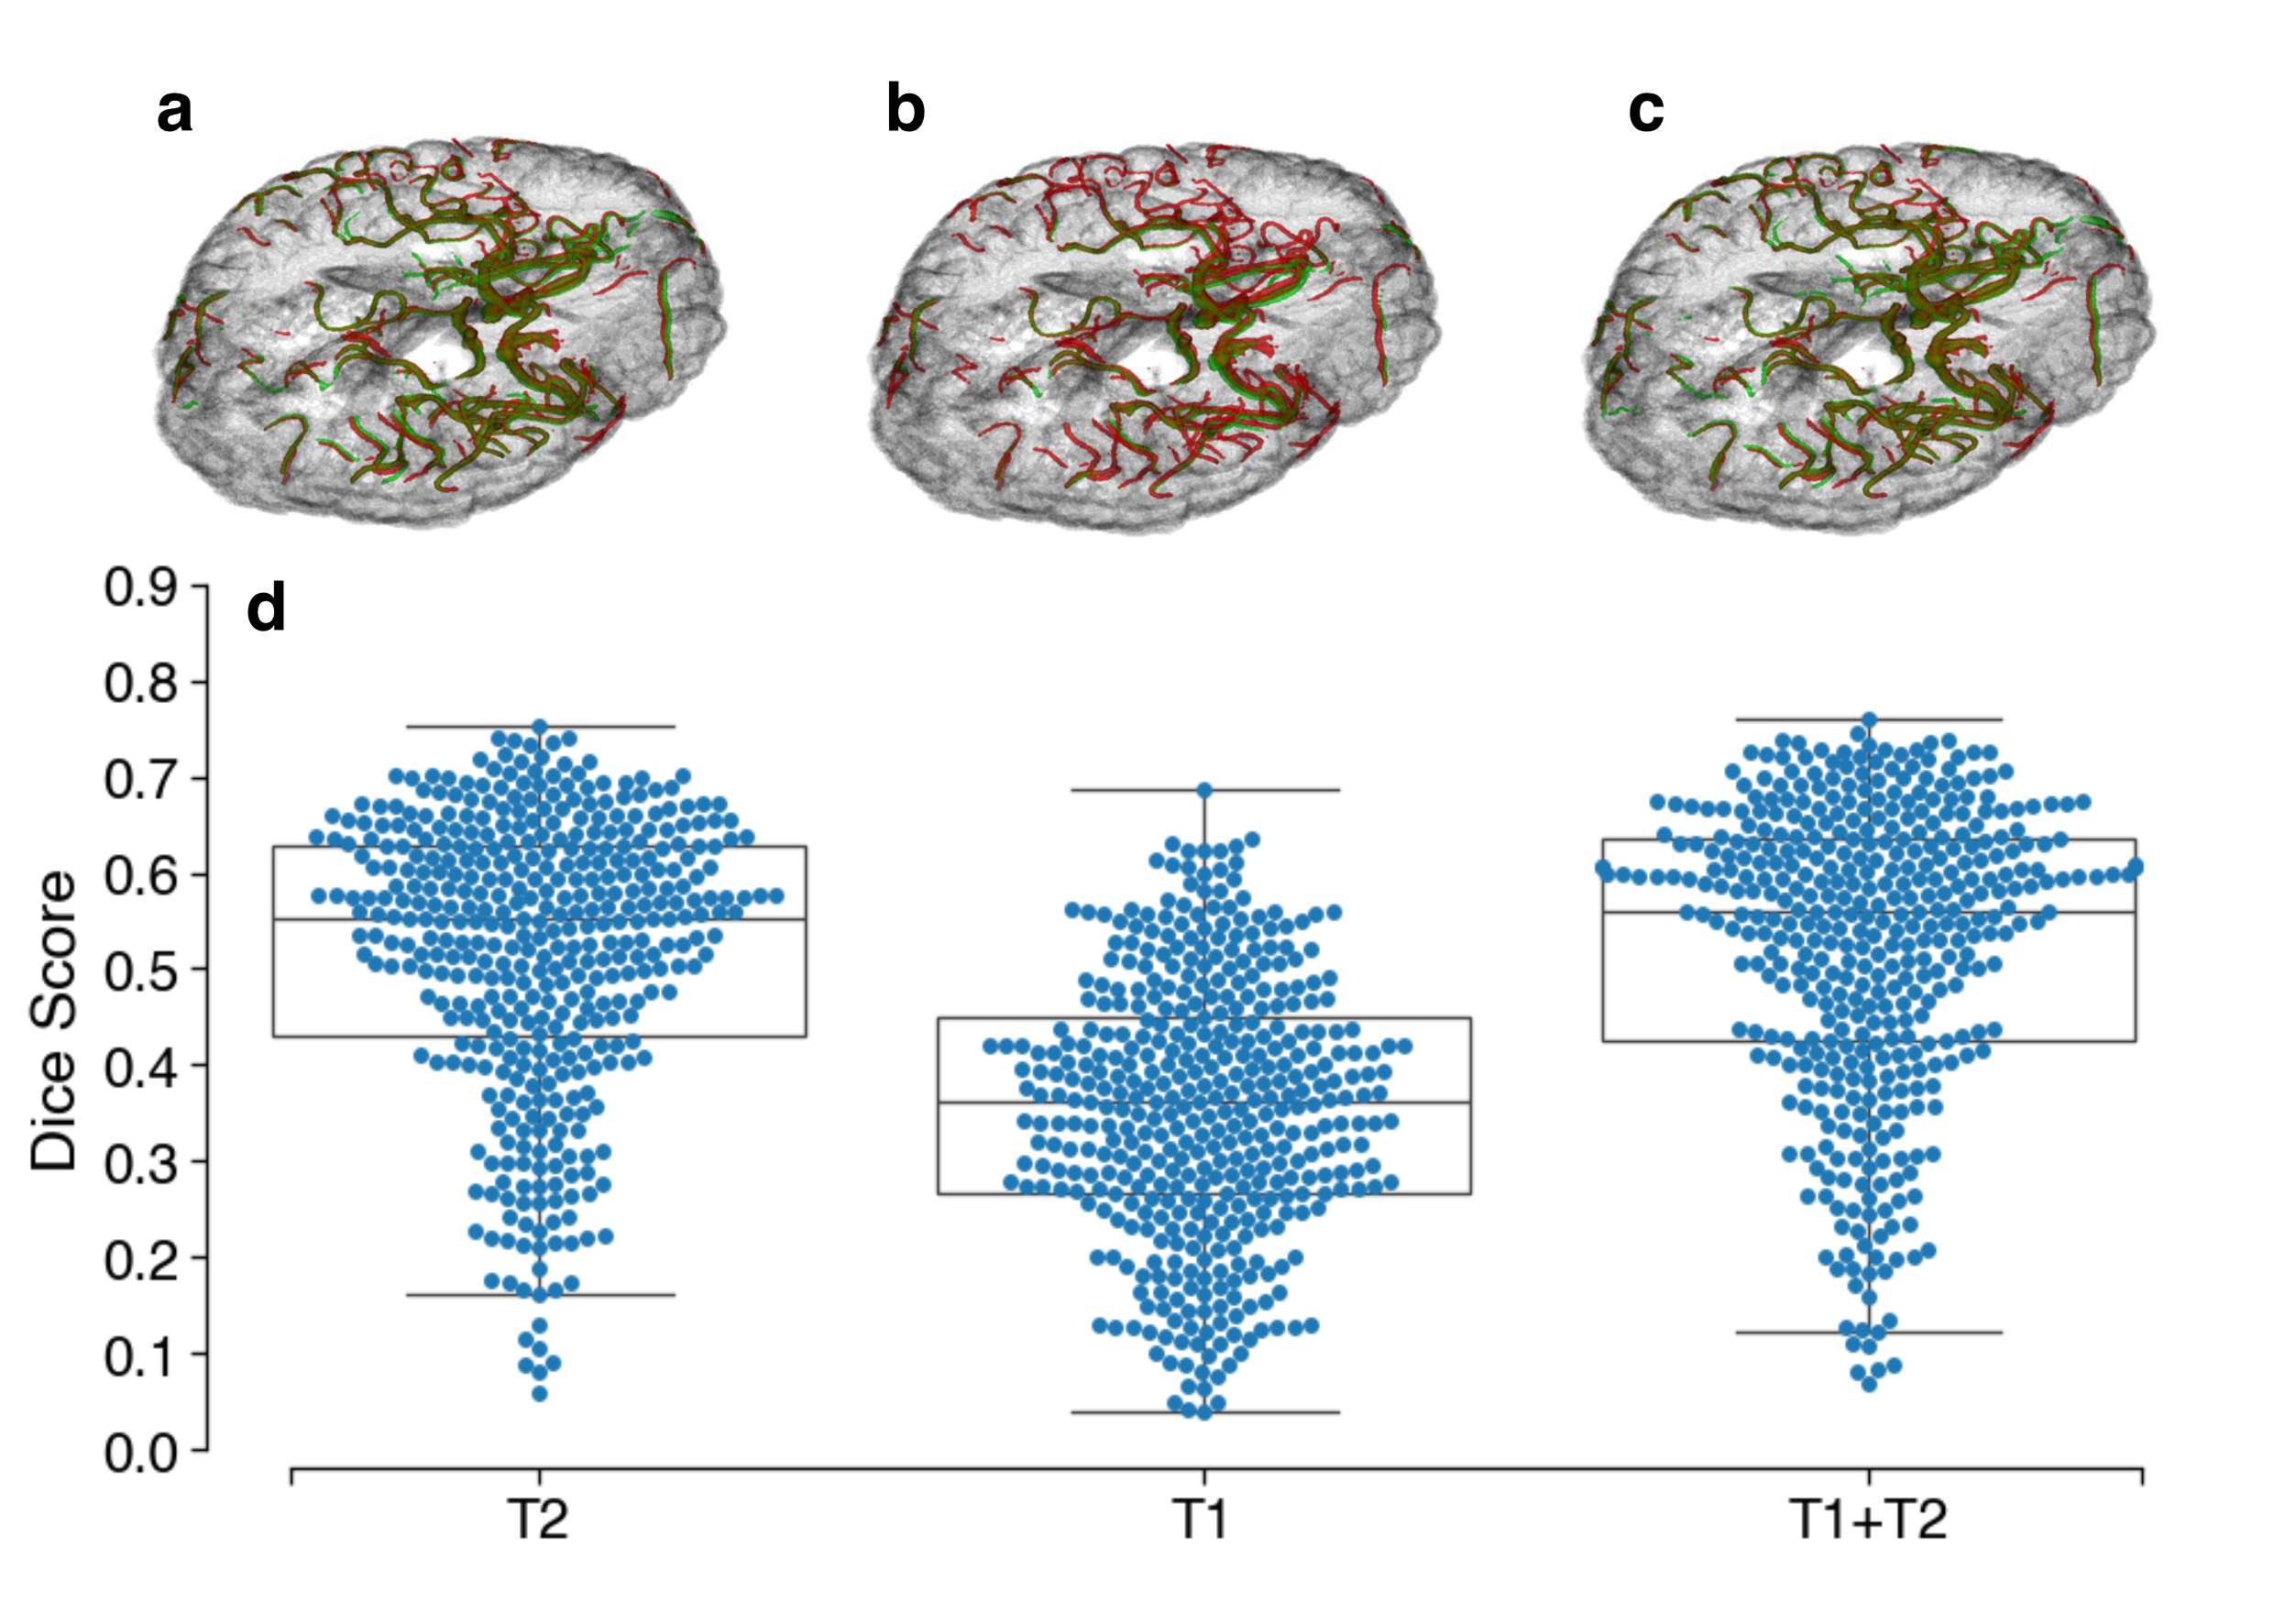
\includegraphics{Figure1.png}
  \end{center}
  \captionof{figure}{Caption for main result. Describe what is shown and highlight key takeaways.}
\end{minipage}
\\

\begin{minipage}[t]{0.8\linewidth}
  % Replace with \includegraphics[width=0.8\linewidth]{secondary-result.png}
  \figplaceholder[10cm]{Secondary result figure}
  \captionof{figure}{Caption for secondary result figure.}
\end{minipage}
\\

\subsection*{Main Result 2: [Descriptive Heading]}

Present your second key result here. Include any statistical tests used and their outcomes
(e.g., Mann–Whitney U test, p\,$<$\,0.05). Relate the result back to your research
question \cite{ref4}.

\begin{minipage}[t]{1.0\linewidth}
  % Replace with \includegraphics[width=0.8\linewidth]{comparison-figure.png}
  \figplaceholder[12cm]{Quantitative comparison figure}
  \captionof{figure}{Quantitative comparison showing [metric] across conditions.}
\end{minipage}
\\

\section*{Additional Applications / Discussion}

\begin{minipage}[t]{1\linewidth}
  % Replace with \includegraphics[width=0.6\linewidth]{application-figure.png}
  \figplaceholder[10cm]{Application or discussion figure}
  \\
  Describe any additional use cases or extensions of your method. Discuss implications,
  limitations, and directions for future work.
\end{minipage}

%------------------------------------------------

\color{SaddleBrown}

\section*{Conclusions}

\begin{itemize}
\large
  \item \textbf{Finding 1:} Concise statement of your first main conclusion.
  \item \textbf{Finding 2:} Concise statement of your second main conclusion.
  \item \textbf{Finding 3:} Broader implications or future directions.
\end{itemize}

\color{DarkSlateGray}

%----------------------------------------------------------------------------
%	REFERENCES
%----------------------------------------------------------------------------
% Dummy references — replace with your own entries or switch to BibTeX:
%   \bibliographystyle{plain}
%   \bibliography{your-bib-file}

\begin{thebibliography}{9}
\footnotesize

\bibitem{ref1}
Author A, Author B.
\textit{Title of Reference 1}.
Journal Name, vol.~X, pp.~1--10, Year.

\bibitem{ref2}
Author C, Author D.
\textit{Title of Reference 2}.
Conference Name, pp.~1--8, Year.

\bibitem{ref3}
Author E.
\textit{Title of Reference 3}.
Journal Name, vol.~Y, pp.~100--110, Year.

\bibitem{ref4}
Author F, Author G, Author H.
\textit{Title of Reference 4}.
Journal Name, vol.~Z, pp.~200--215, Year.

\end{thebibliography}

%----------------------------------------------------------------------------

\end{multicols}
\end{document}